\documentclass[a4paper,12pt]{article}

\input{"$HOME/Desktop/Studia/LaTeX/setup.tex"}

\author{Wojciech Orłowski}
\title{\textsc{Generatory liczb pseudolosowych o zadanym rozkładzie w jednym
wymiarze} - sprawozdanie}

\begin{document}
    \maketitle

    \section{Wstęp}

    Jednym z podstawowych narzędzi potrzebnych do symulacji Monte Carlo jest możliwość wygenerowania zmiennej losowej o zadanej funkcji gęstości prawdopodobieństwa.
    Istnieją różne metody, aby generowania takich liczb.
    Zwykle korzystają one z ogólnodostępnych generatorów jednorodnych.
    W badanych przypadkach chcemy uzyskać liczby o rozkładzie fgp (funkcji gęstości prawdopodobieństwa) opisanej równaniem \eqref{fgp}
    \begin{equation}
        f(x) = \frac{4}{5}(1 + x - x^3),
        \label{fgp}
    \end{equation}
    i dystrybuancie opisanej równaniem \eqref{dst}
    \begin{equation}
        F(x) = \frac{4}{5}\left(x + \frac{x^2}{2} - \frac{x^4}{4}\right).
        \label{dst}
    \end{equation}
    \\
    \\
    Celem ćwiczenia jest zapoznanie studentów z metodami generowania liczb pseudolosowych o zadanym rozkładzie oraz ich porównanie.
    Metody implementowane podczas ćwiczenia wykorzystują generator liniowy o rozkładzie jednorodnym. 
    Tymi metodami są:
    \begin{itemize}
        \item metoda rozkładu złożonego,
        \item metoda łańcucha Markowa,
        \item metoda eliminacji.
    \end{itemize}
    W metodzie rozkładu złożonego dystrybuante zapisujemy jako sumę dwóch wielomianów.
    Następnie znajdujemy funkcję odwrotne do tych wielomianów.
    Jedną z wylosowanych liczb wykorzystamy aby określić z którego z wielomianu skorzystamy do generacji liczby o zadanym rozkładzie.
    Druga jest wykorzystana do bezpośredniej generacji liczby pseudolosowej.
    \\
    \\
    W metodzie wykorzystującej łańcuchy Markowa generujemy ciąg liczb pseudolosowych, w której określamy prawdopodobieństwo okreslenia nowego stanu.
    Ponadto proponowany stan jest zależny od parametru $\Delta$, należy także zatem przeanalizować wpływ tego parametru na wygenerowany ciąg.
    \\
    \\
    Metoda eliminacji jest metodą losowania, w której ograniczamy funkcję gęstości prawdopodobieństwa odgórnie inną funkcją.
    Musimy znać generator liczb o rozkładzie tej funkcji.
    Generowane są dwie liczby, jedna o rozkładzie jednorodnym ($U$), a druga o rozkładzie ograniczającym ($G$).
    Zwracana jest $U$, jeżeli spełniony jest warunek $(G \leq f(U))$.
    Obliczenia wykonywane były w języku \julia.

    \section{Wyniki}

    Skonstruowane zostały histogramy dla wylosowanych $N = 10^6$ liczb pseudolosowych o zadanym rozkładzie.
    Histogramy zostały podzielone na 10 przedziałów oraz znormalizowane.
    
    \begin{figure}[h]
        \centering
        \begin{subfigure}{0.49\textwidth}
            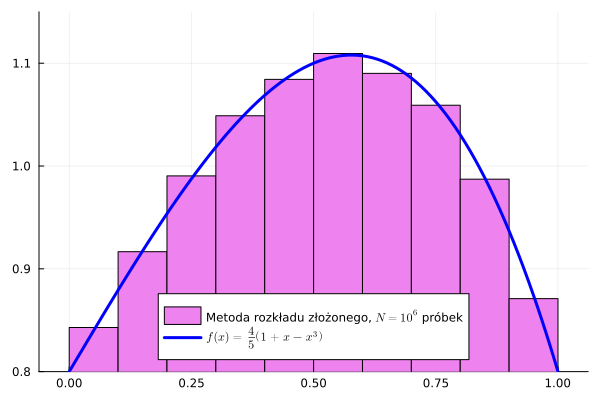
\includegraphics[width=\textwidth]{../gallery/compound.png}
            \caption{}
        \end{subfigure}
        \begin{subfigure}{0.49\textwidth}
            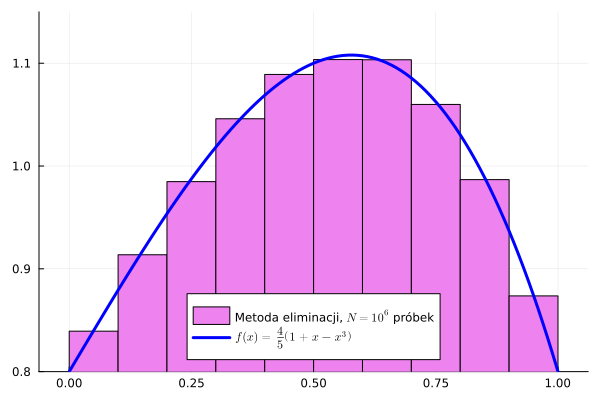
\includegraphics[width=\textwidth]{../gallery/elimination.png}
            \caption{}
        \end{subfigure}
        \\
        \begin{subfigure}{0.49\textwidth}
            \includegraphics[width=\textwidth]{../gallery/markov_005.png}
            \caption{}
        \end{subfigure}
        \begin{subfigure}{0.49\textwidth}
            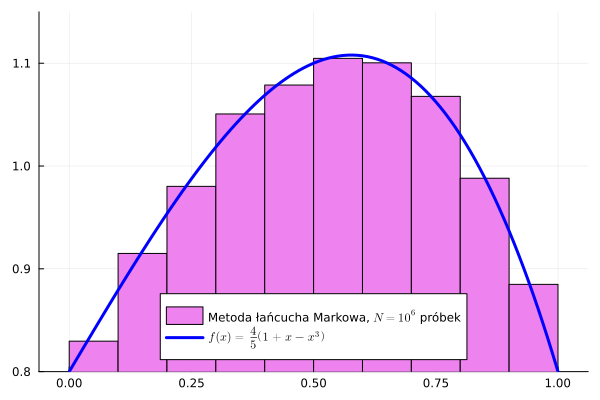
\includegraphics[width=\textwidth]{../gallery/markov_05.png}
            \caption{}
        \end{subfigure}
        \caption{Histogramy dla trzech metod generowania liczb pseudolosowych 
        o dystrybuancie $F(x)$. (a) Metoda rozkładu złożonoego, (b) metoda eliminacji,
        (c) łańcuch Markowa z $\Delta$ = 0.05, (d) łańcuch Markowa z $\Delta$ = 0.5.}
    \end{figure}

    \noaka Dla każdej z metod możemy zauważyć, że histogram jest zbliżony do właściwej funkcji gęstości prawdopodobieństwa.
    Aby porównać te metody w sposób analityczny trzeba wykonać test statystyczny, np. test $\chi^2$.
    Gołym okiem możemy natomiast stwierdzić, że histogram dla łańcucha Markowa z $\Delta = 0.05$ najbardziej odbiega od fgp.
    Jest on lekko przesunięty w lewo. 
    \\
    \\
    Rozważania ilościowe dotyczące wylosowanych zestawów można porównać korzystając z testu statystycznego.
    W teście $\chi^2$ dla poziomu ufności $0.95$ dla 9 stopni swobody wartość krytyczna tego testu wynosi 16.919.
    W celu dokładniejszego porównania, takich testów zostało wykonanych 5 dla każdego zestawu, a ich wyniki zostały przedstawione poniżej (rys. \ref{chi}).
   
    \begin{figure}[H]
        \centering
        \begin{subfigure}{0.49\textwidth}
            \begin{verbatim}
        (5.689319255809376, true)
        (7.546540110026232, true)
        (6.482566016197022, true)
        (8.436397294213297, true)
        (8.439572763078058, true)
            \end{verbatim}       
            \caption{}    
        \end{subfigure}
        \begin{subfigure}{0.49\textwidth}
            \begin{verbatim}
    (1.9718807158628695, true)
    (8.930059114966706, true)
    (5.0384531835351005, true)
    (6.334742767769672, true)
    (6.049185777097399, true)
            \end{verbatim}       
            \caption{}    
        \end{subfigure}
        \\
        \begin{subfigure}{0.49\textwidth}
            \begin{verbatim}
    (142.04229167800517, false)
    (616.1348467620983, false)
    (512.630939675032, false)
    (1158.0403233328582, false)
    (1527.1207839886372, false)
            \end{verbatim}       
            \caption{}    
        \end{subfigure}
        \begin{subfigure}{0.49\textwidth}
            \begin{verbatim}
    (16.40976416512897, true)
    (19.90712421687445, false)
    (27.818970905668763, false)
    (16.26503847384019, true)
    (19.979460274140237, false)
            \end{verbatim}       
            \caption{}    
        \end{subfigure}

        \caption{Porównanie testów $\chi^2$, dla (a) metody rozkładu złożonego, (b) metody eliminacji, (c) łańcucha Markowa $\Delta$ = 0.05, (d) łańcucha Markowa $\Delta =  0.5$. Wykonano po 5 testów dla każdej z metod, przedstawiona wartość logiczna odpowiada czy wartość $\chi^2$ mieści się w statystyce testowej.}
        \label{chi}
    \end{figure}

    \noaka Dla metod rozkładu złożonego i eliminacji wszystkie wartości $\chi^2$ mieszczą się w statystyce testowej.
    Dla metody wykorzystującej łańcuchy Markowa z wartością $\Delta = 0.5$ nie wszystkie wartości $\chi^2$ są mniejsze od wartości krytycznej.
    Natomiast dla mniejszej wartości $\Delta$ równej 0.05 żadne losowanie nie mieści się w statystyce testowej. 
    Ponadto wartości te bardzo odbiegają od wartości krytycznej oraz są od niej wielokrotnie większe.     
    \\
    \\
    Do analizy pozostaje jeszcze czas obliczeń. 
    Korzystając z makra języka \julia $\,$ \texttt{@time} można w prosty sposób przeanalizować czasy przeprowadzanych losowań.
    Dla metody rozkładu złożonego czas ten wyniósł
    \begin{verbatim}
        0.130901 seconds (4.00 M allocations: 76.278 MiB, 10.17% gc time),
    \end{verbatim}
    dla metody eliminacji
    \begin{verbatim}
        0.124228 seconds (4.00 M allocations: 76.278 MiB, 6.02% gc time),
    \end{verbatim}
    a dla metody wykorzystującej łańcuchy Markowa
    \begin{verbatim}
        0.075945 seconds (3.05 M allocations: 54.135 MiB, 2.58% gc time).
    \end{verbatim}
    Zatem po szybkiej analizie można stwierdzić, że metoda wykorzystująca łańcuchy Markowa jest szybsza od pozostałych.
    Metody eliminacji i rozkładu złożonego trwają porównywalnie tyle samo czasu.
    \\
    \\
    Porównując z sobą metody generujące łańcuch Markowa dla różnych parametrów $\Delta$ otrzymujemy histogram przedstawiony na rys. \ref{markow2}.
    \begin{figure}[H]
        \centering
        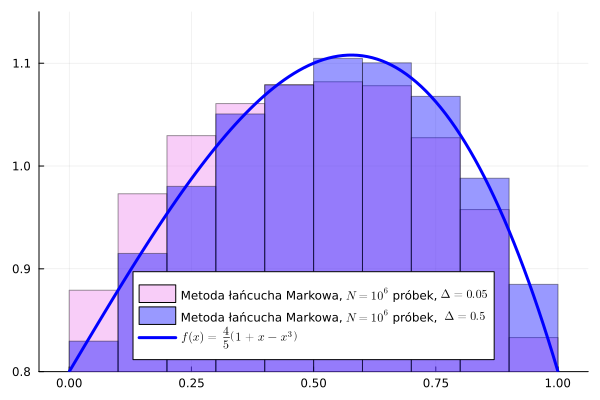
\includegraphics[width=0.7\textwidth]{../gallery/markov_05_005.png}
        \caption{Porównanie histogramów dla wygenerowanych zestawów metodą łańcucha Markowa.}
        \label{markow2}
    \end{figure}
    
    \noaka Analizując ten histogram możemy stwierdzić, że dla niskiego parametru $\Delta$ dane są mało zgodne z funkcją gęstości prawdopodobieństwa.
    Są one przesunięte lekko w lewo.
    Natomiast wygenerowane liczby dla $\Delta = 0.5$ są bardziej zgodne, jednak porównując je z testem $\chi^2$ widzimy, że wciąż nie są bardzo dokładne i czasami nie spełniają wartości krytycznej dla przedziału ufności $0.95$.

    \section{Podsumowanie}

    Podczas zajęć laboratoryjnych udało się wygenerować zestawy liczb pseudolosowych o zadanym rozkładzie korzystając z różnych metod.
    Przeanalizowano także wpływ parametru na zgodność wygenerowanego rozkładu w metodzie łańcuchów Markowa.
    Widać, że parametr ten musi być dobrany optymalnie, wykonując wcześniej pewną ilość losowań.
    Najszybszą metodą losowania okazała się metoda wykorzystująca łańcuchy Markowa, jednak dla tej metody powstały również największe błędy średniokwadratowe.
    Metody eliminacji i rozkładu złożonego trwały dłużej, jednak przy każdym losowaniu statystyka testowa $\chi^2$ była mniejsza od wartości krytycznej.
 

\end{document}
